\begin{figure}
  \centering
  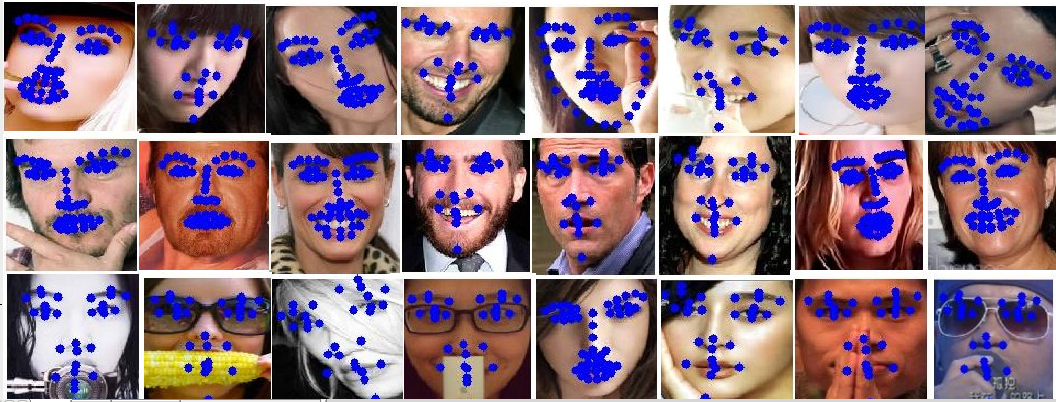
\includegraphics[width=6in,height=2in]{fid/figures/pose_expression_occlusion.png}
  \caption{Results with varying pose (Row 1), expression (Row 2) and 
  occlusion (Row 3). Best viewed in color.}
  \label{fig:sample_results}
\end{figure}

\label{subsec:quant}

\begin{figure*}[!ht]
  \centering
  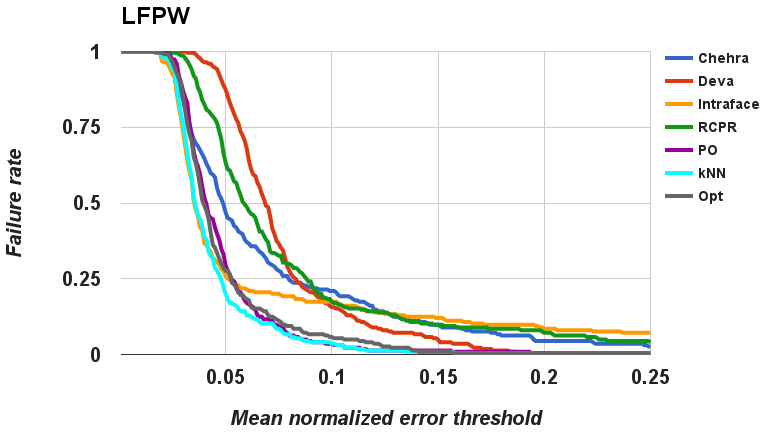
\includegraphics[width=4.8in,height=2.4in]{fid/figures/lfpw_failure_rate_graph.png}
  \caption{Results of our approach on (a) LFPW, (b) COFW, and (c) AFLW datasets.
  Drop in failure rate with the change in cut-off threshold of mean error normalized 
  with interocular distance. Lower curve means more accurate results. Best viewed in color.}
  \label{fig:graph_results}
  % On x-axis, we plot increasing value 
  % of mean normalized error, which is the mean of pixel error normalized by interocular distance.
  % On y-axis, we plot the fraction of images with greater error.}
\end{figure*}

\begin{figure*}[!ht]
  \centering
  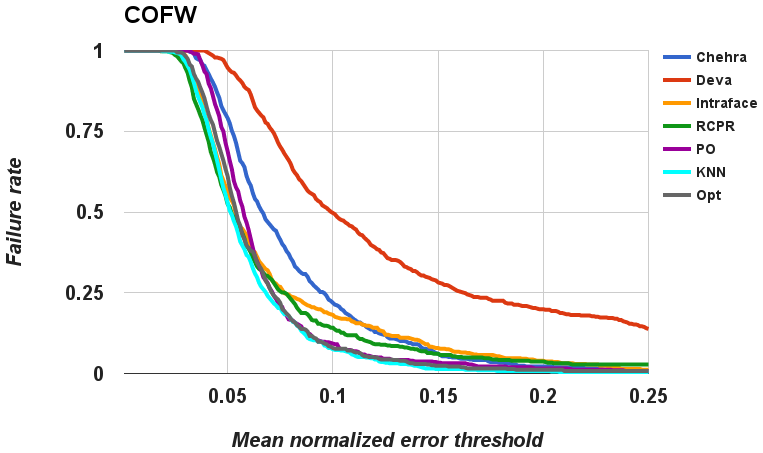
\includegraphics[width=4.8in,height=2.4in]{fid/figures/cofw_failure_rate_graph.png}
  \caption{Results of our approach on (a) LFPW, (b) COFW, and (c) AFLW datasets.
  Drop in failure rate with the change in cut-off threshold of mean error normalized 
  with interocular distance. Lower curve means more accurate results. Best viewed in color.}
  \label{fig:graph_results}
  % On x-axis, we plot increasing value 
  % of mean normalized error, which is the mean of pixel error normalized by interocular distance.
  % On y-axis, we plot the fraction of images with greater error.}
\end{figure*}

\begin{figure*}[!ht]
  \centering
  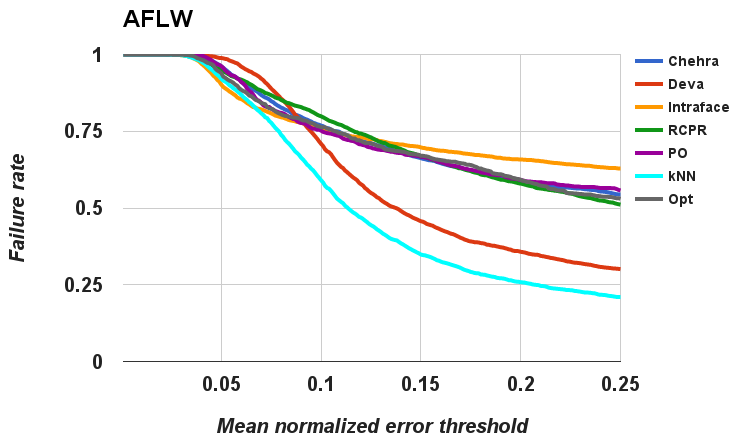
\includegraphics[width=4.8in,height=2.4in]{fid/figures/aflw_failure_rate_graph.png}
  \caption{Results of our approach on (a) LFPW, (b) COFW, and (c) AFLW datasets.
  Drop in failure rate with the change in cut-off threshold of mean error normalized 
  with interocular distance. Lower curve means more accurate results. Best viewed in color.}
  \label{fig:graph_results}
  % On x-axis, we plot increasing value 
  % of mean normalized error, which is the mean of pixel error normalized by interocular distance.
  % On y-axis, we plot the fraction of images with greater error.}
\end{figure*}

In this section, we outline the basis for future
experiments detailed in the next sections.
Table~\ref{table:ourBestResults_mean} shows
results of our approach on LFPW, COFW and AFLW datasets. To produce these results, we first
resize \emph{all} images (training and testing) to a size of $300 \times 300$, and 
compute a set of $20$ exemplars for each dataset using Algorithm~\ref{alg:exemplar_selection},
equally divided between shape and appearance. Figure~\ref{fig:cofw_lfpw_exemplars} illustrates our
results of exemplar selection on the LFPW dataset. SIFT features for each fiducial are calculated at
the scale of $5$ and $8$ pixels, which roughly translates to $4\%$ and and $6\%$ of the
interocular distance. Once this is done, we proceed to the output selection by kNN and optimization
based algorithms. 
%For each given test image, we first run all the candidate algorithms and store their outputs. For each
%output, we then compute its distance in feature space to the selected exemplars, and choose the
%exemplar with minimum distance (kNN with $k=1$). We finally choose the output that has the minimum
%distance to its nearest exemplar. 
  
\begin{table}%[!h]
   \centering
   \begin{tabular}{c c c c c c c c}
    \toprule[1.5pt]
%    & \multicolumn{6}{c}{Mean Error} & & & \multicolumn{6}{c}{Failure Rate} \\
%    \toprule[0.5pt]
%     \specialcell{\bf Dataset} &  \specialcell{\bf Chehra} &  \specialcell{\bf \textcolor{red}{Zhu}} &  \specialcell{\bf Intraface} &  \specialcell{\bf RCPR} &  \specialcell{\bf Ours} \\
     {\bf Dataset} &  {\bf Chehra} &  {\bf Zhu} &  {\bf Intraface} &  {\bf RCPR} & {\bf PO} & {\bf Ours} & {\bf Ours} \\
     & & & & & & \bf(kNN) & \bf(Opt) \\
    \midrule
    {\bf LFPW} &  7.21 & 7.60 & 7.79 & 9.28 & {\bf 4.82} & {\bf 4.31 } & 4.83 \\ 
    {\bf COFW} &  7.95 & 15.76 & 7.22 & 7.30 & 6.73 &{\bf 5.98 } & {\bf 6.28} \\
    {\bf AFLW} &  40.44 & {\bf 25.88} & 47.98 & 39.78 & 46.67 & {\bf 19.93} & 32.08 \\ 
    \bottomrule[1.5pt]
%     \specialcell{\bf Dataset} &  \specialcell{\bf Chehra} &  \specialcell{\bf \textcolor{red}{Zhu}} &  \specialcell{\bf Intraface} &  \specialcell{\bf RCPR} &  \specialcell{\bf Ours} \\

    \end{tabular}
    \caption{Table shows the mean error and failure rate for three datasets. In each row, top two algorithms are highlighted for both mean error and failure rate. Opt in the table represents output selection by optimization. Observe that both of our algorithms consistently perform better than state-of-the-art algorithms. }
    \label{table:ourBestResults_mean}
\end{table}

\begin{table}%[!h]
   \centering
   \begin{tabular}{c c c c c c c c}
    \toprule[1.5pt]
    %& \multicolumn{6}{c}{Mean Error} & & & \multicolumn{6}{c}{Failure Rate} \\
%    \toprule[0.5pt]
%     \specialcell{\bf Dataset} &  \specialcell{\bf Chehra} &  \specialcell{\bf \textcolor{red}{Zhu}} &  \specialcell{\bf Intraface} &  \specialcell{\bf RCPR} &  \specialcell{\bf Ours} \\
     {\bf Dataset} & {\bf Chehra} & {\bf Zhu} & {\bf Intraface} & {\bf RCPR} & {\bf PO} & {\bf Ours} & {\bf Ours }\\
     & & & & & & \bf(kNN) & \bf(Opt) \\%& & & & & & \bf(kNN) & \bf(Opt)\\
    \midrule
    {\bf LFPW} &  20.98 & 15.62 & 17.41 & 17.41 & {\bf 3.57} &{\bf 3.57} & 5.8 \\ 
    {\bf COFW} &  21.89 & 49.70 & 18.15 & 14.20 & 9.27 &{\bf 7.49 } & {\bf 7.88} \\
    {\bf AFLW} &  80.52 & {\bf 71.28} & 79.80 & 82.12 & 75.20 & {\bf 59.03} & 76.30  \\ 
    \bottomrule[1.5pt]
%     \specialcell{\bf Dataset} &  \specialcell{\bf Chehra} &  \specialcell{\bf \textcolor{red}{Zhu}} &  \specialcell{\bf Intraface} &  \specialcell{\bf RCPR} &  \specialcell{\bf Ours} \\

    \end{tabular}
    \caption{Table shows the mean error and failure rate for three datasets. In each row, top two algorithms are highlighted for both mean error and failure rate. Opt in the table represents output selection by optimization. Observe that both of our algorithms consistently perform better than state-of-the-art algorithms. }
    \label{table:ourBestResults_fail}
\end{table}

For each test dataset in Table~\ref{table:ourBestResults_mean}, 
mean errors and failure rates in locating fiducials over the entire dataset are shown. For each fiducial, we first compute
the ratio of its Euclidean distance from the ground truth and the interocular distance for that
image. We then average this ratio over the entire image and over the entire dataset. Thus the first
table represents the \emph{average ratio of fiducial error and interocular distance over the entire
dataset}. The failure rate is the
fraction of images in the entire dataset, for which this ratio is more than $0.1$ 
($10 \%$ error). Thus, while mean error gives an idea of the accuracy of our algorithm, the
failure rate gives an idea of its robustness. 
 
A more detailed quantitative comparison of our approach with candidate algorithms is
presented in Figure~\ref{fig:graph_results}.
Each point on the x-axis of this figure represents a cut-off threshold, and each corresponding
point on the y-axis of this figure represents the fraction of images that have 
mean normalized error greater than this cut-off. Thus, graphs that dip quickly are 
more accurate.
% This figure depicts the change in failure rate with the 
% change in cut-off threshold of mean normalized error 
% for different datasets. 
The mean normalized error is the mean of all interocular distance
normalized errors over the entire dataset. 
We notice that both of our algorithms consistently perform better 
compared to other five algorithms at almost all cut-off ranges.
Figure~\ref{fig:sample_results} illustrates some qualitative results using our approach.

